\documentclass[11pt]{article}
\usepackage[margin=1in]{geometry}

\usepackage{amsmath}
\usepackage{amssymb}
\usepackage[utf8]{inputenc} 
\usepackage{graphicx} 
\usepackage{parskip} 
\usepackage{multirow} 
\usepackage{mathtools}

\DeclarePairedDelimiter\abs{\lvert}{\rvert}%
\DeclarePairedDelimiter\norm{\lVert}{\rVert}%

\makeatletter
\let\oldabs\abs
\def\abs{\@ifstar{\oldabs}{\oldabs*}}

\let\oldnorm\norm
\def\norm{\@ifstar{\oldnorm}{\oldnorm*}}
\makeatother
\usepackage{multicol} 
\usepackage[spanish,es-nodecimaldot]{babel} 
\usepackage{mathtools}
\usepackage{amsfonts}
\usepackage{float}
\usepackage{textcomp}
\usepackage{caption}
\usepackage{subfig}
\usepackage[spanish]{babel}
\usepackage{gensymb}
\def\sen{\mathop{\mbox{\normalfont sen}}\nolimits}

\usepackage{fancyhdr}
\fancyhf{}
\rfoot{\thepage}
\pagestyle{fancy}
\lhead{Nieto Castellanos Jaime Fabián}
\chead{}
\rhead{Tarea 8. Histogramas}
\begin{document}

\textbf{1)}
\begin{figure}[H]
\centering
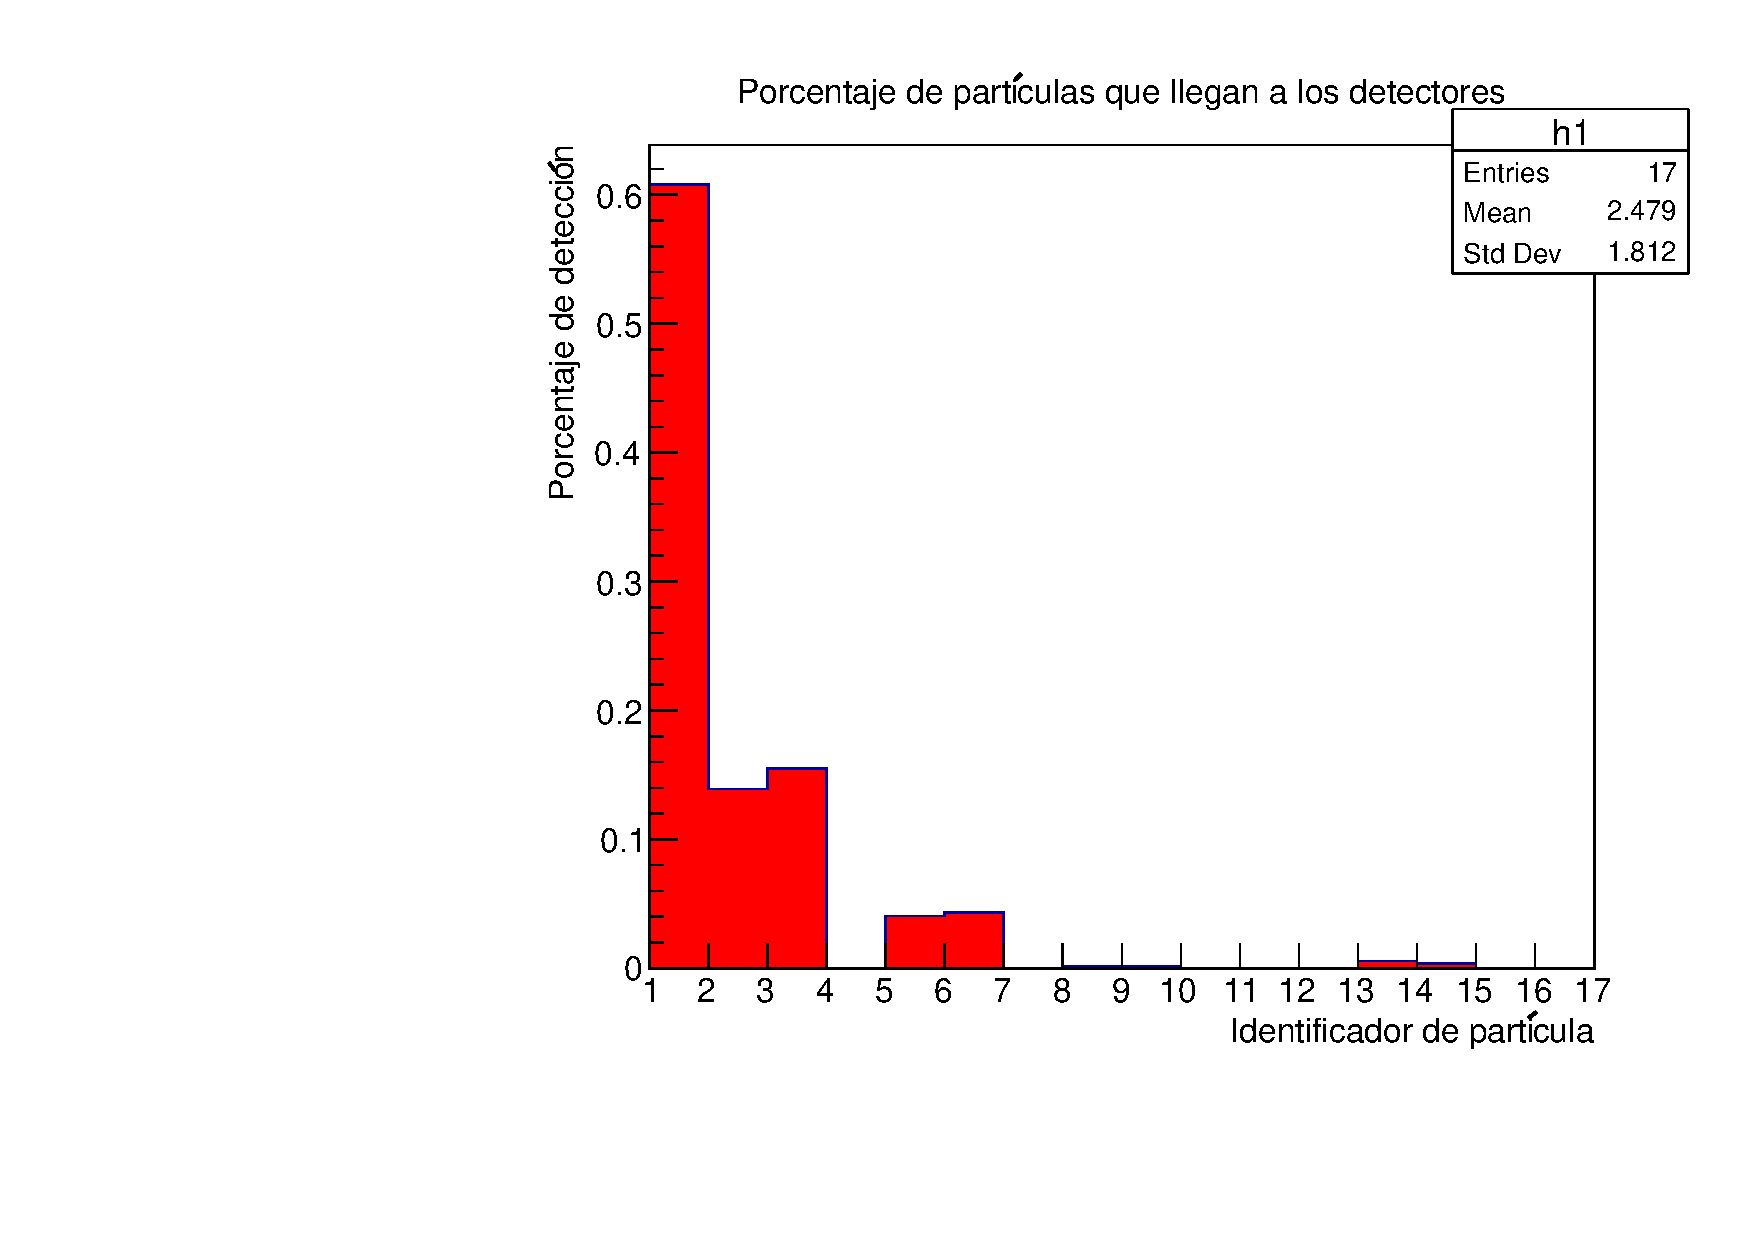
\includegraphics[width=0.7\textwidth]{../Figuras/Prob1A.pdf}
\caption{ Porcentaje de cada tipo de partícula que llega a los detectores de HAWC. El 1 significa $\gamma$, el 2 $e^+$ y el 3 $e^-$}
\label{fig:Prob1A}
\end{figure}
Para separar el conjunto de datos en tres rangos energéticos, lo haremos considerando la integral de la distribución de energía, figura \ref{fig:Prob1B}. Si el área debajo del histograma es $A$, entonces el primer rango de energías corresponde a la primera tercera parte del área, el segundo rango corresponde a la segunda tercera parte del área y el tercer rango corresponde a la última. Los detalles se encuentran en el archivo Prob1.C. Después de realizar el procedimiento anterior, los rangos en los que dividimos nuestro conjunto de datos son [0,2500GeV), [2500GeV,8500GeV) y [8500GeV, 1e5 GeV]. En la figura \ref{fig:Prob1C} se observa que el resultado es prácticamente el mismo en los tres rangos energéticos.


\begin{figure}[H]
\centering
{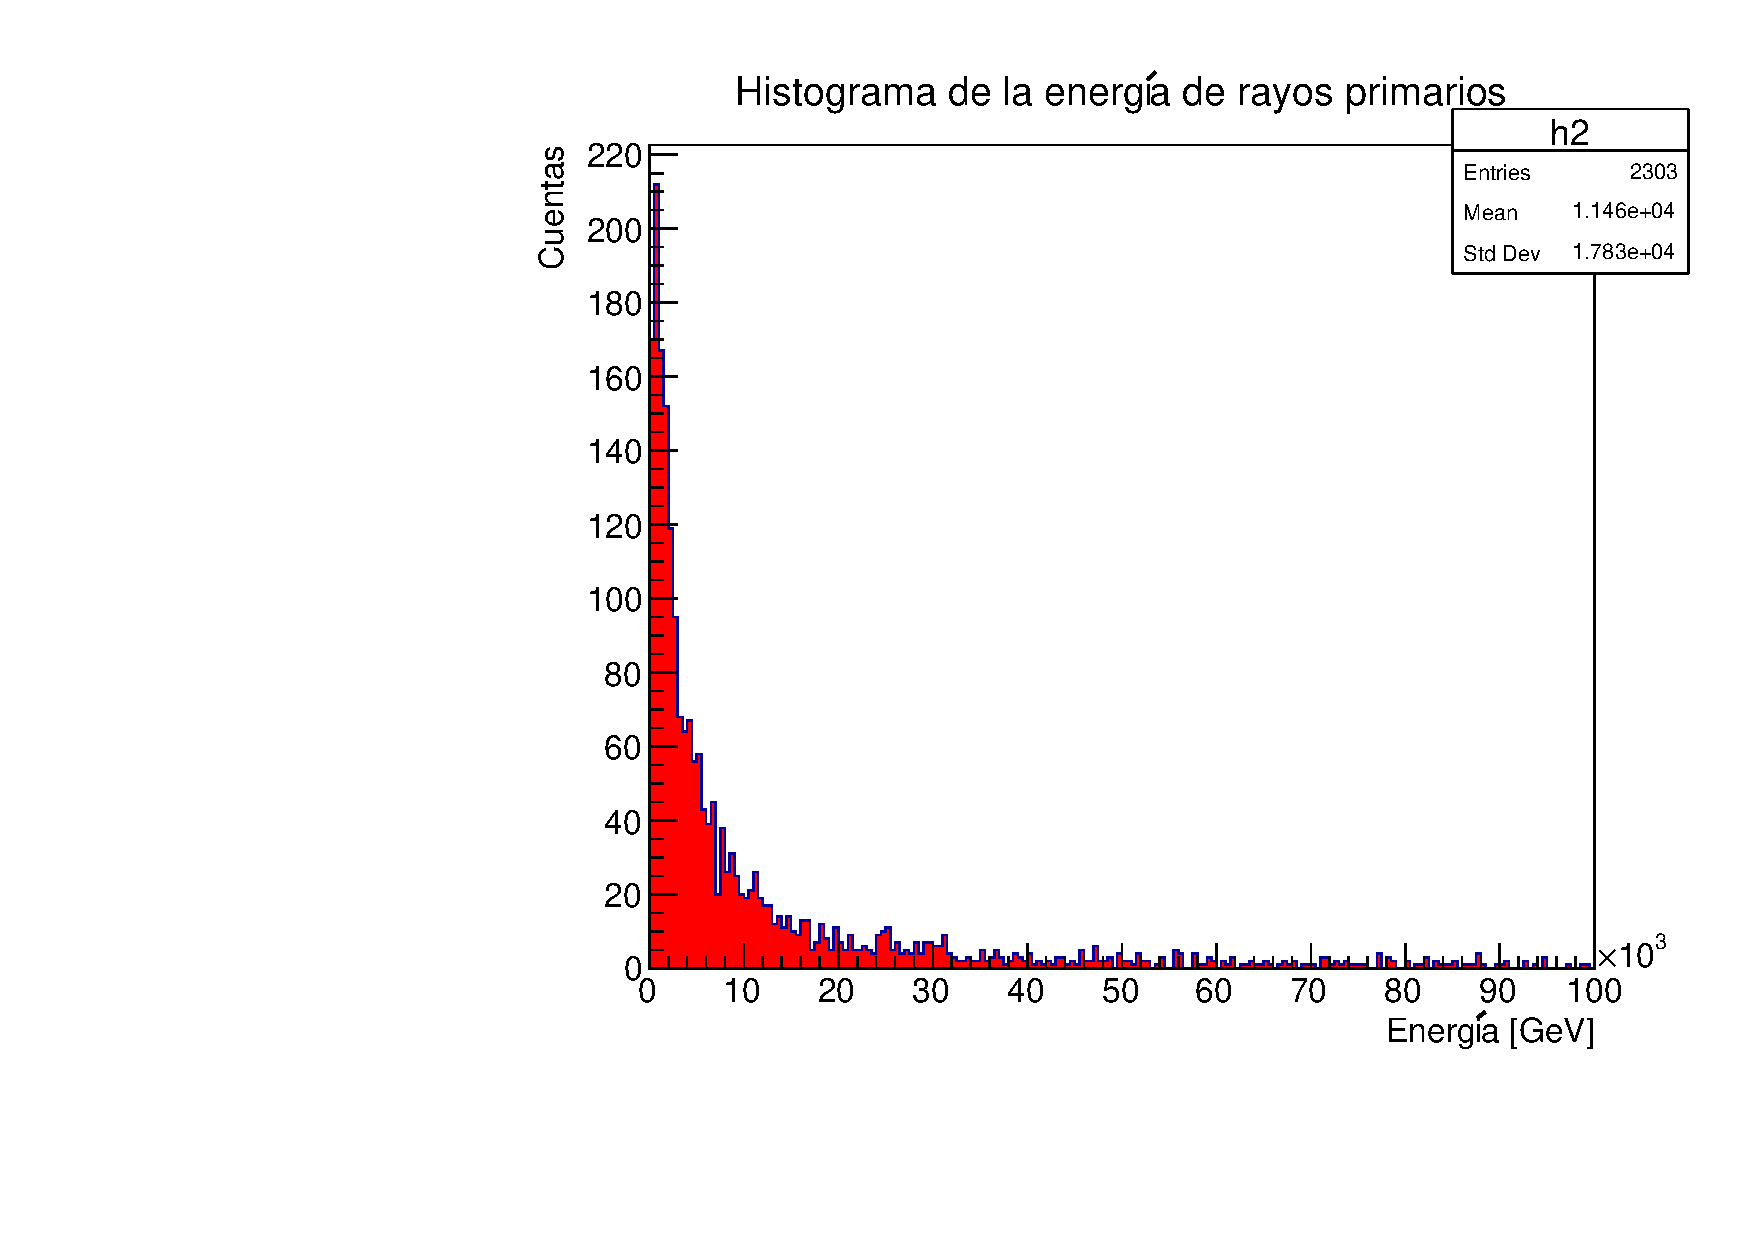
\includegraphics[width=0.7\textwidth]{../Figuras/Prob1B.pdf}}
\caption{ Histograma de la distribución de energía del archivo de datos.}
\label{fig:Prob1B}
\end{figure}


\begin{figure}[H]
\centering
\subfloat[\centering Intervalo [0,2500GeV)]{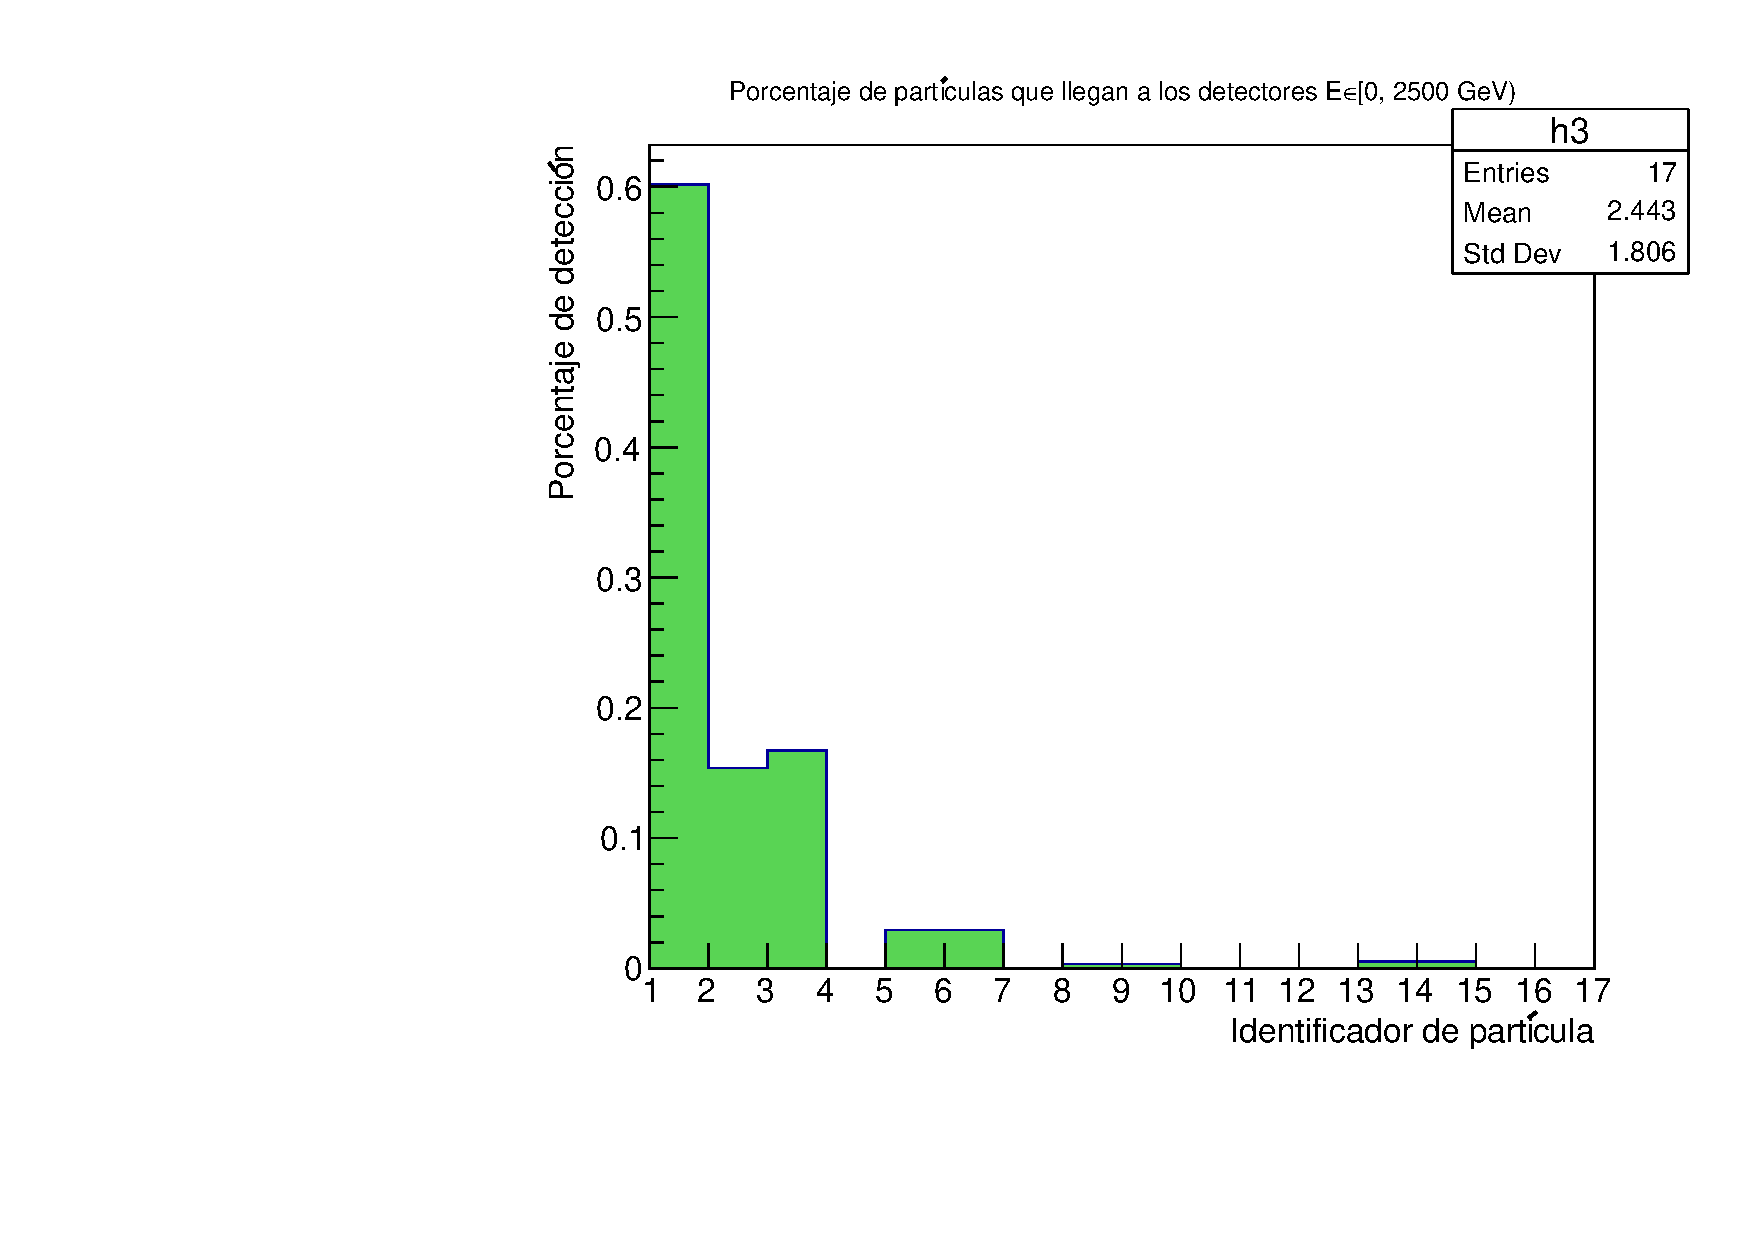
\includegraphics[width=0.7\textwidth]{../Figuras/Prob1C1.pdf}}
\end{figure}

\begin{figure}[H]
\centering
\subfloat[\centering Intervalo [2500GeV,8500GeV)]{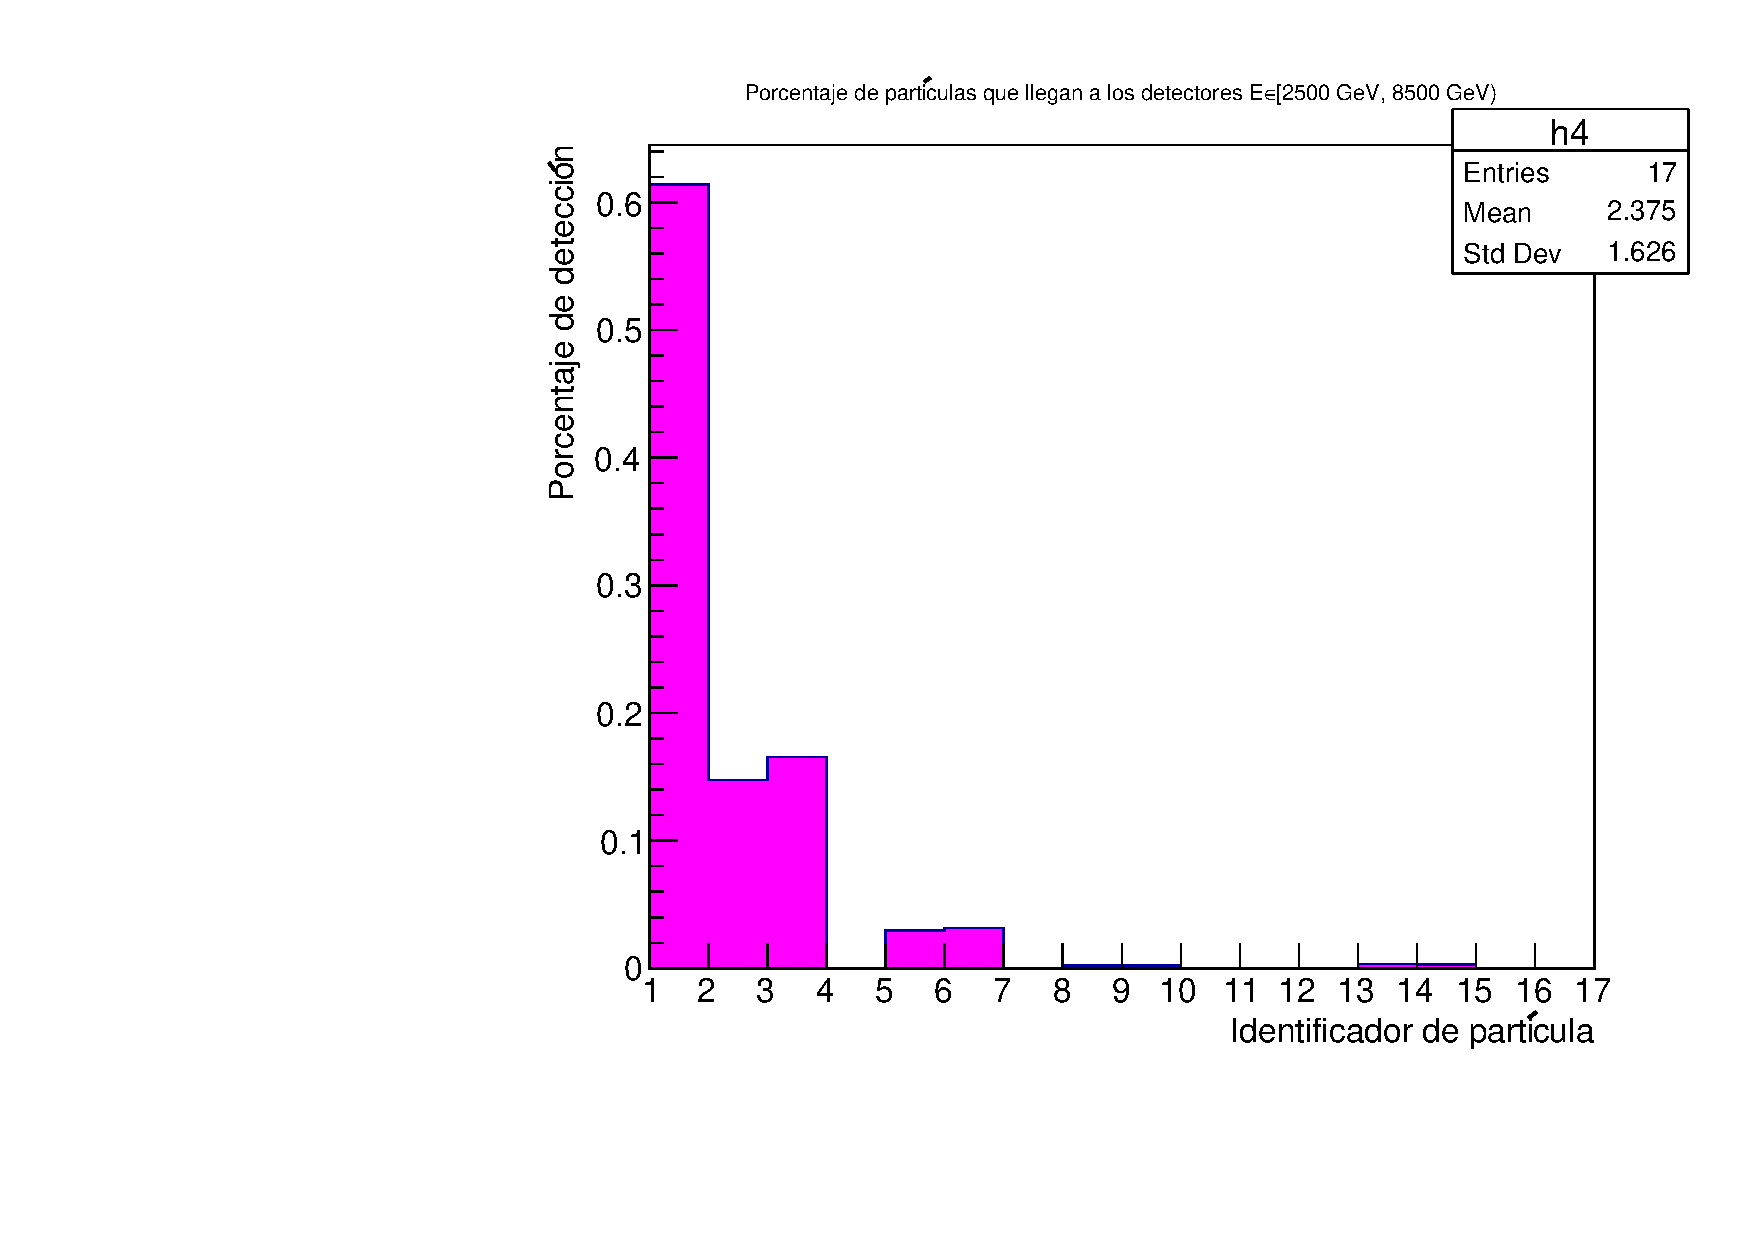
\includegraphics[width=0.7\textwidth]{../Figuras/Prob1C2.pdf}}

\subfloat[\centering Intervalo [8500GeV, 1e5 GeV)]{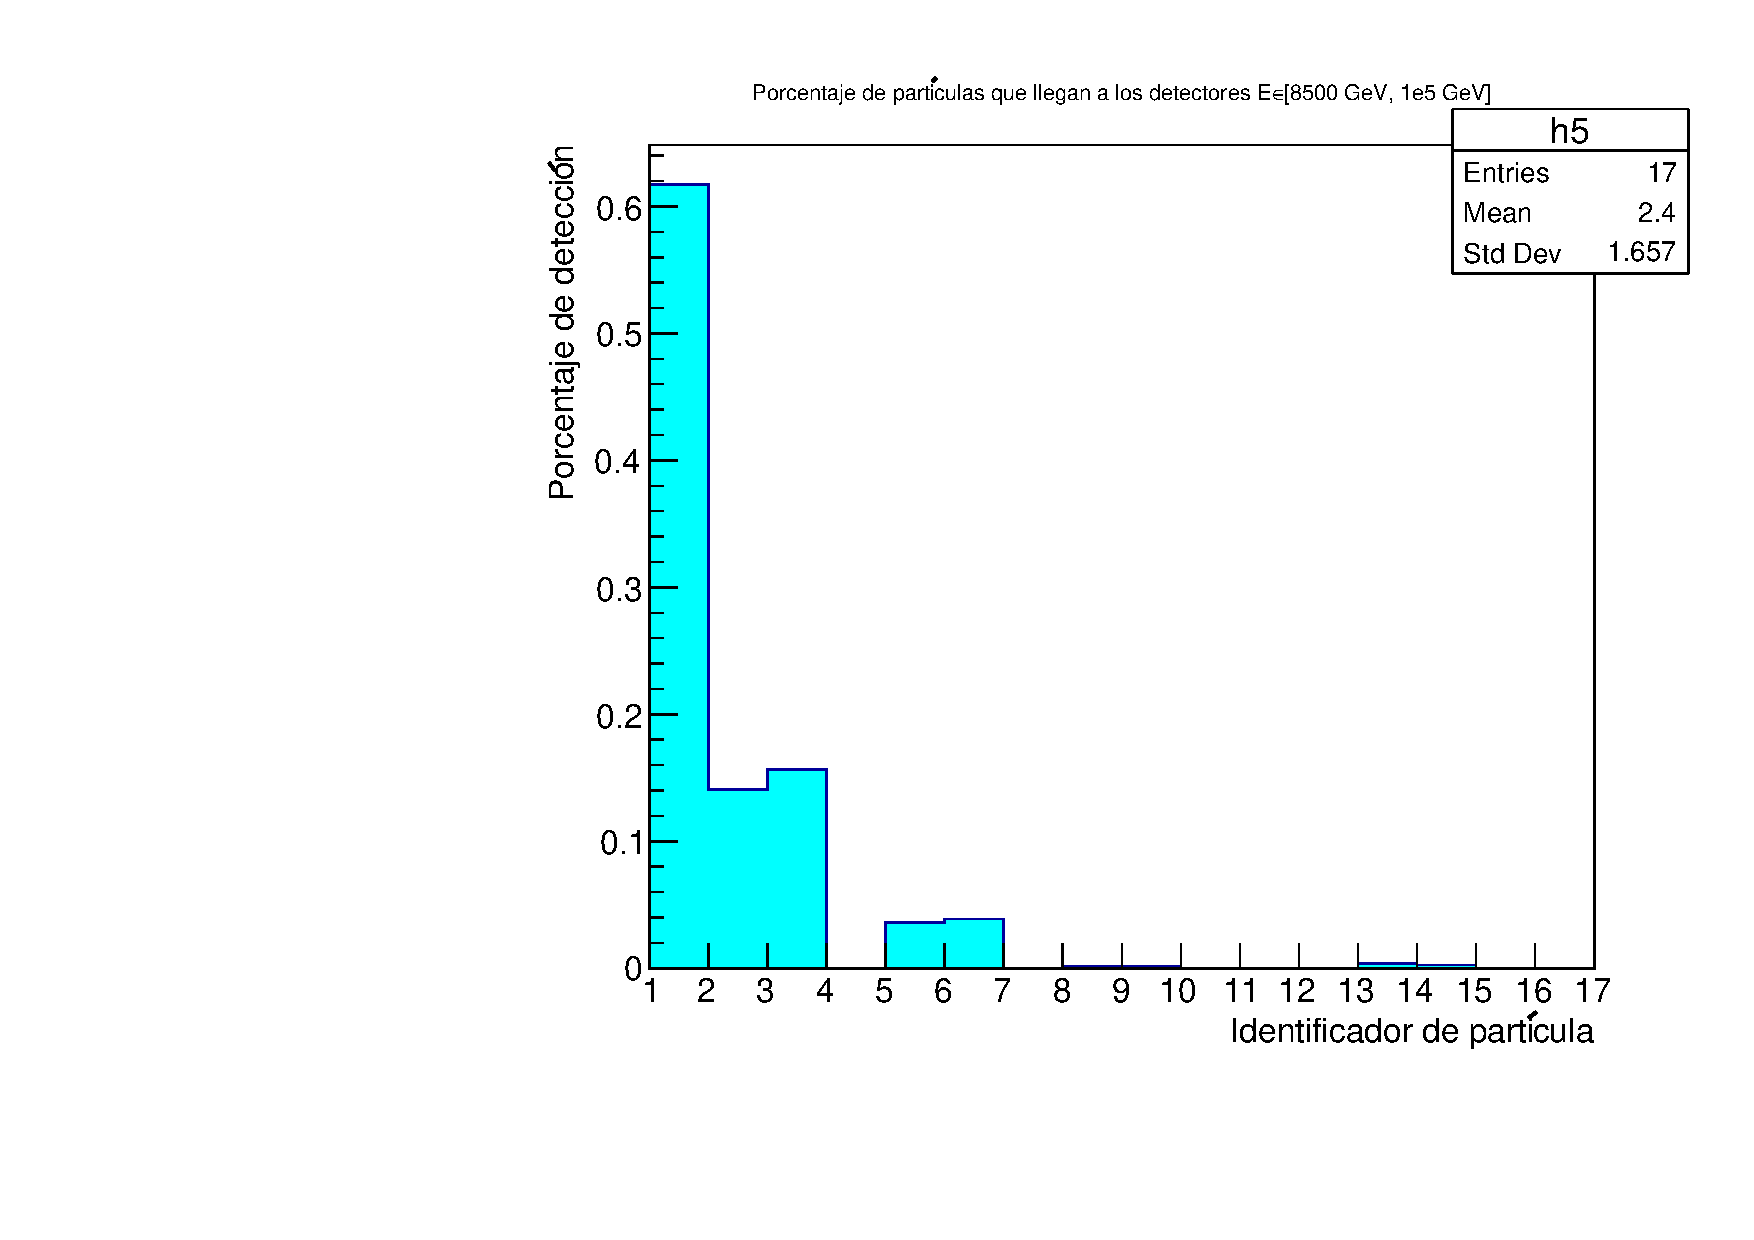
\includegraphics[width=0.7\textwidth]{../Figuras/Prob1C3.pdf}}
\caption{Porcentaje de partículas de cada tipo que llega a los detectores de HAWC para diferentes rangos energéticos con el mismo número de estadística.}
\label{fig:Prob1C}
\end{figure}
\pagebreak
%%%%%%%%%%%%%%%%%%%%%%%%%%%%%%%%%%%%%%%%%%%%%%%%
\textbf{2)} Mostramos la distribución lateral para los eventos 1, 25 y 198.
\begin{figure}[H]
\centering
\subfloat[\centering Evento 1]{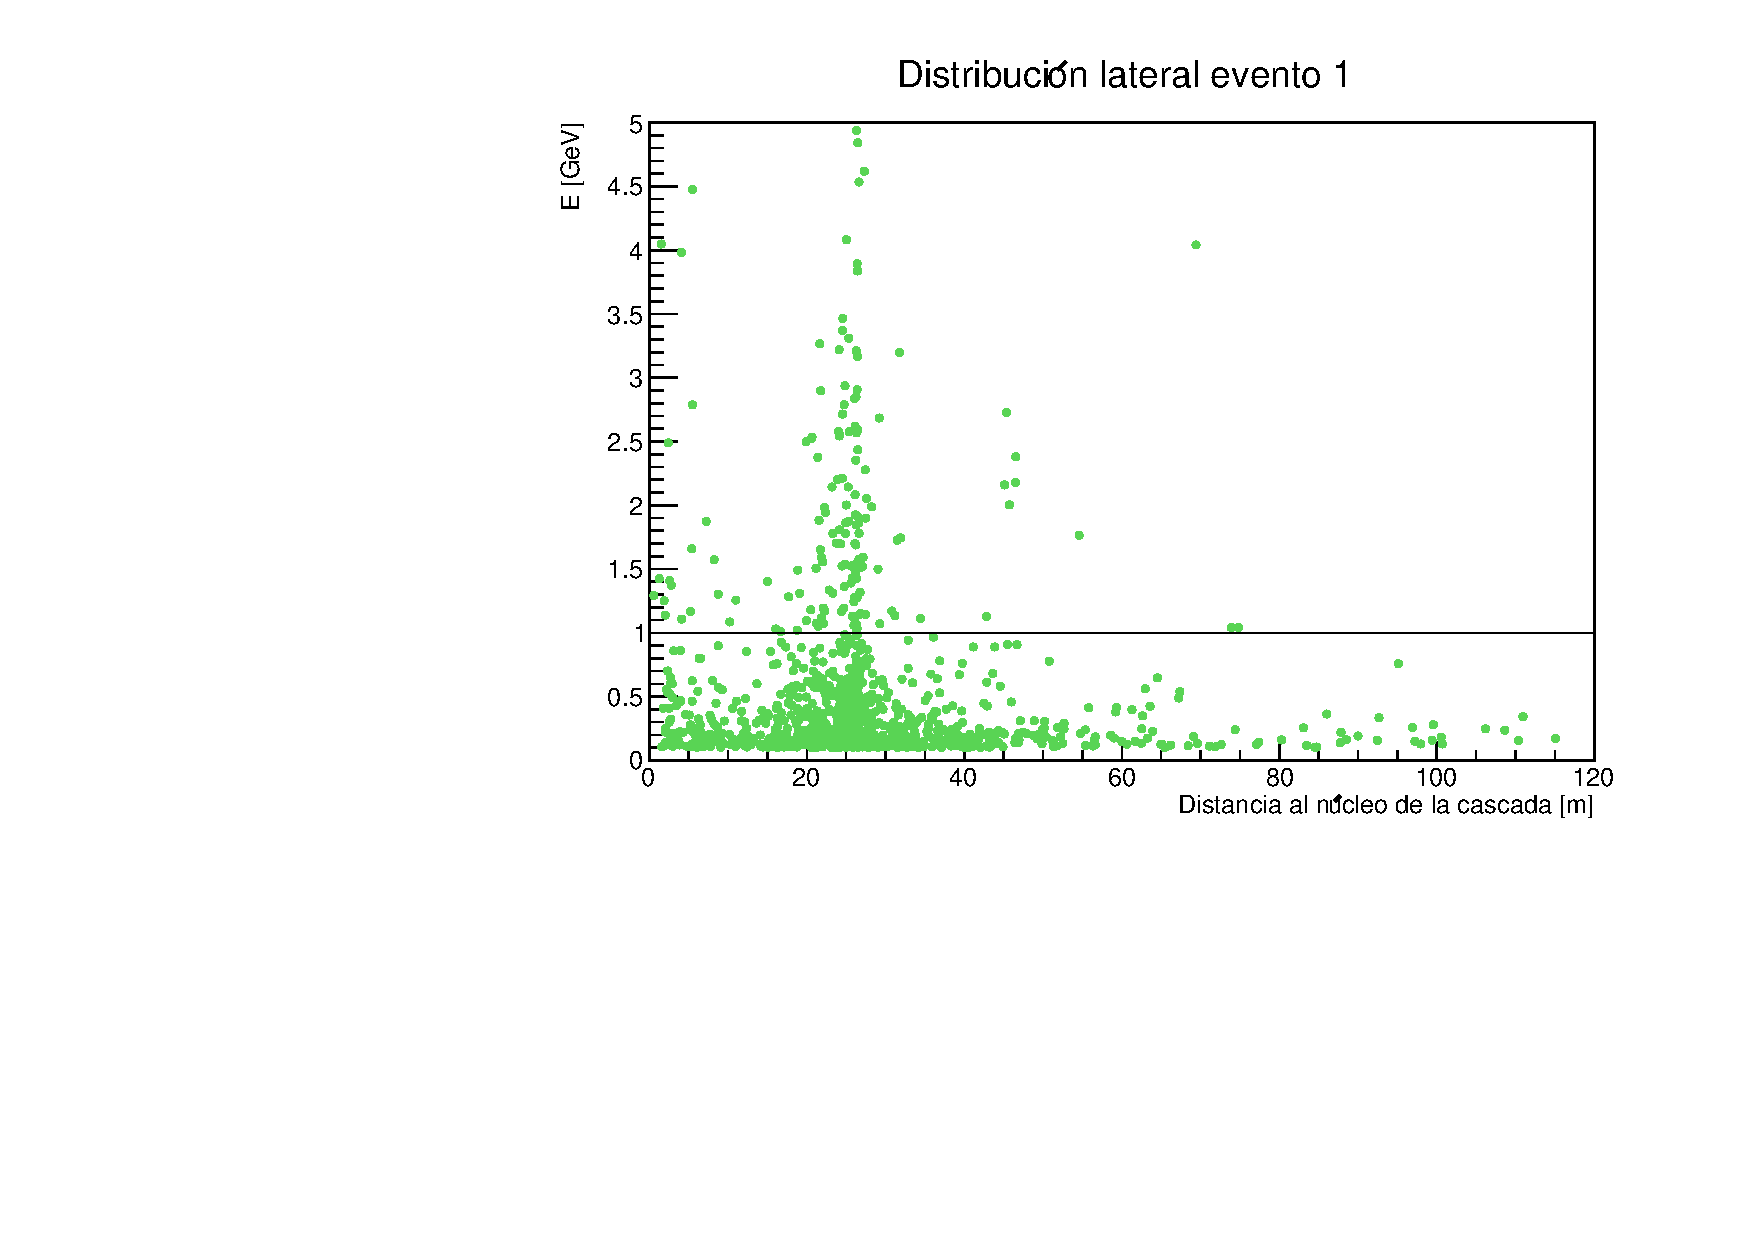
\includegraphics[width=0.9\textwidth]{../Figuras/Prob2A.pdf}}

\subfloat[\centering Evento 25]{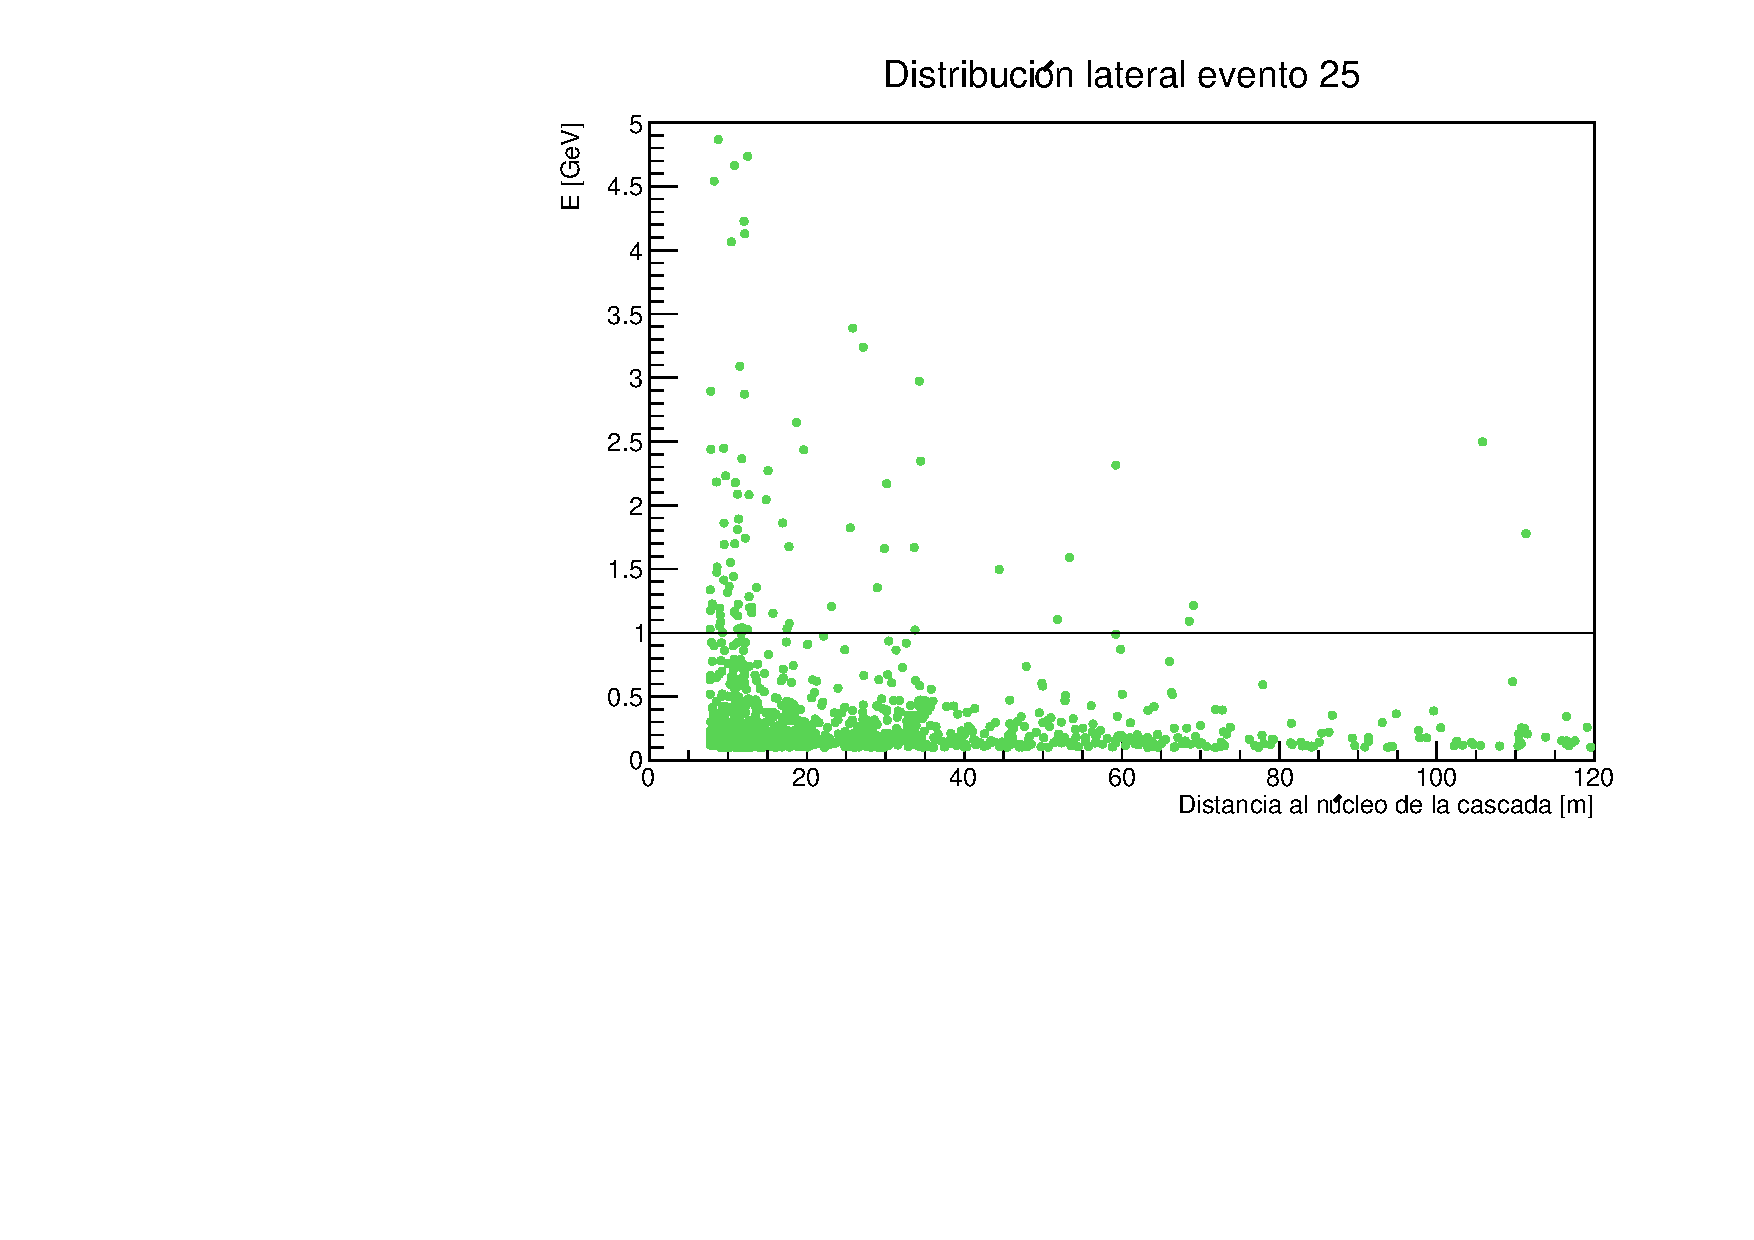
\includegraphics[width=0.9\textwidth]{../Figuras/Prob2B.pdf}}
\end{figure}

\begin{figure}[H]
\centering 
\subfloat[\centering Evento 198]{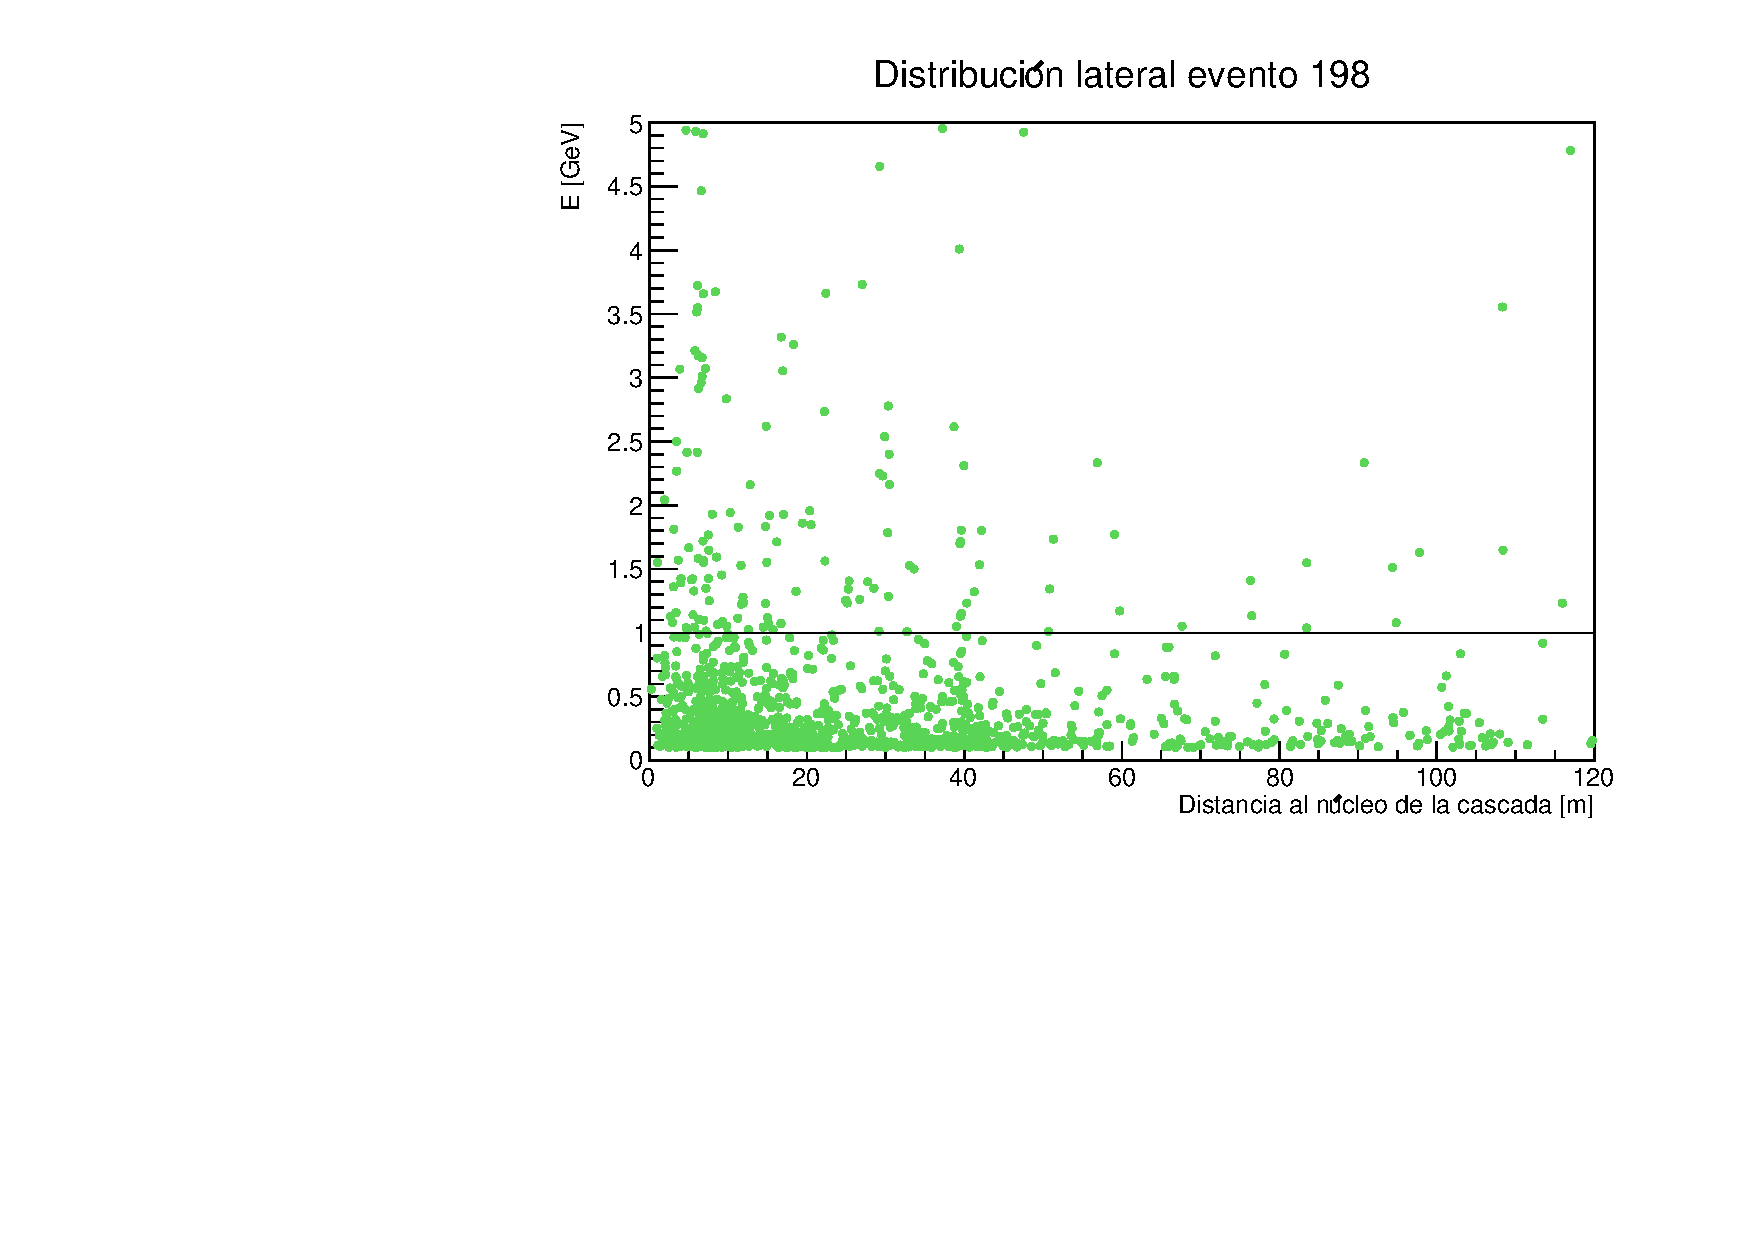
\includegraphics[width=0.9\textwidth]{../Figuras/Prob2C.pdf}}
\caption{Distribución lateral para distintos eventos. Estos eventos satisfacen tener más de 70 hits con un mínimo de 70 GeV.}
\label{fig:Prob2A}
\end{figure}
De los eventos anteriores elegimos el evento 198 para separar la distribución lateral para las tres partículas más abundantes que llegan a los detectores. El resultado se muestra en la figura \ref{fig:Prob2B}.
\begin{figure}[H]
\centering
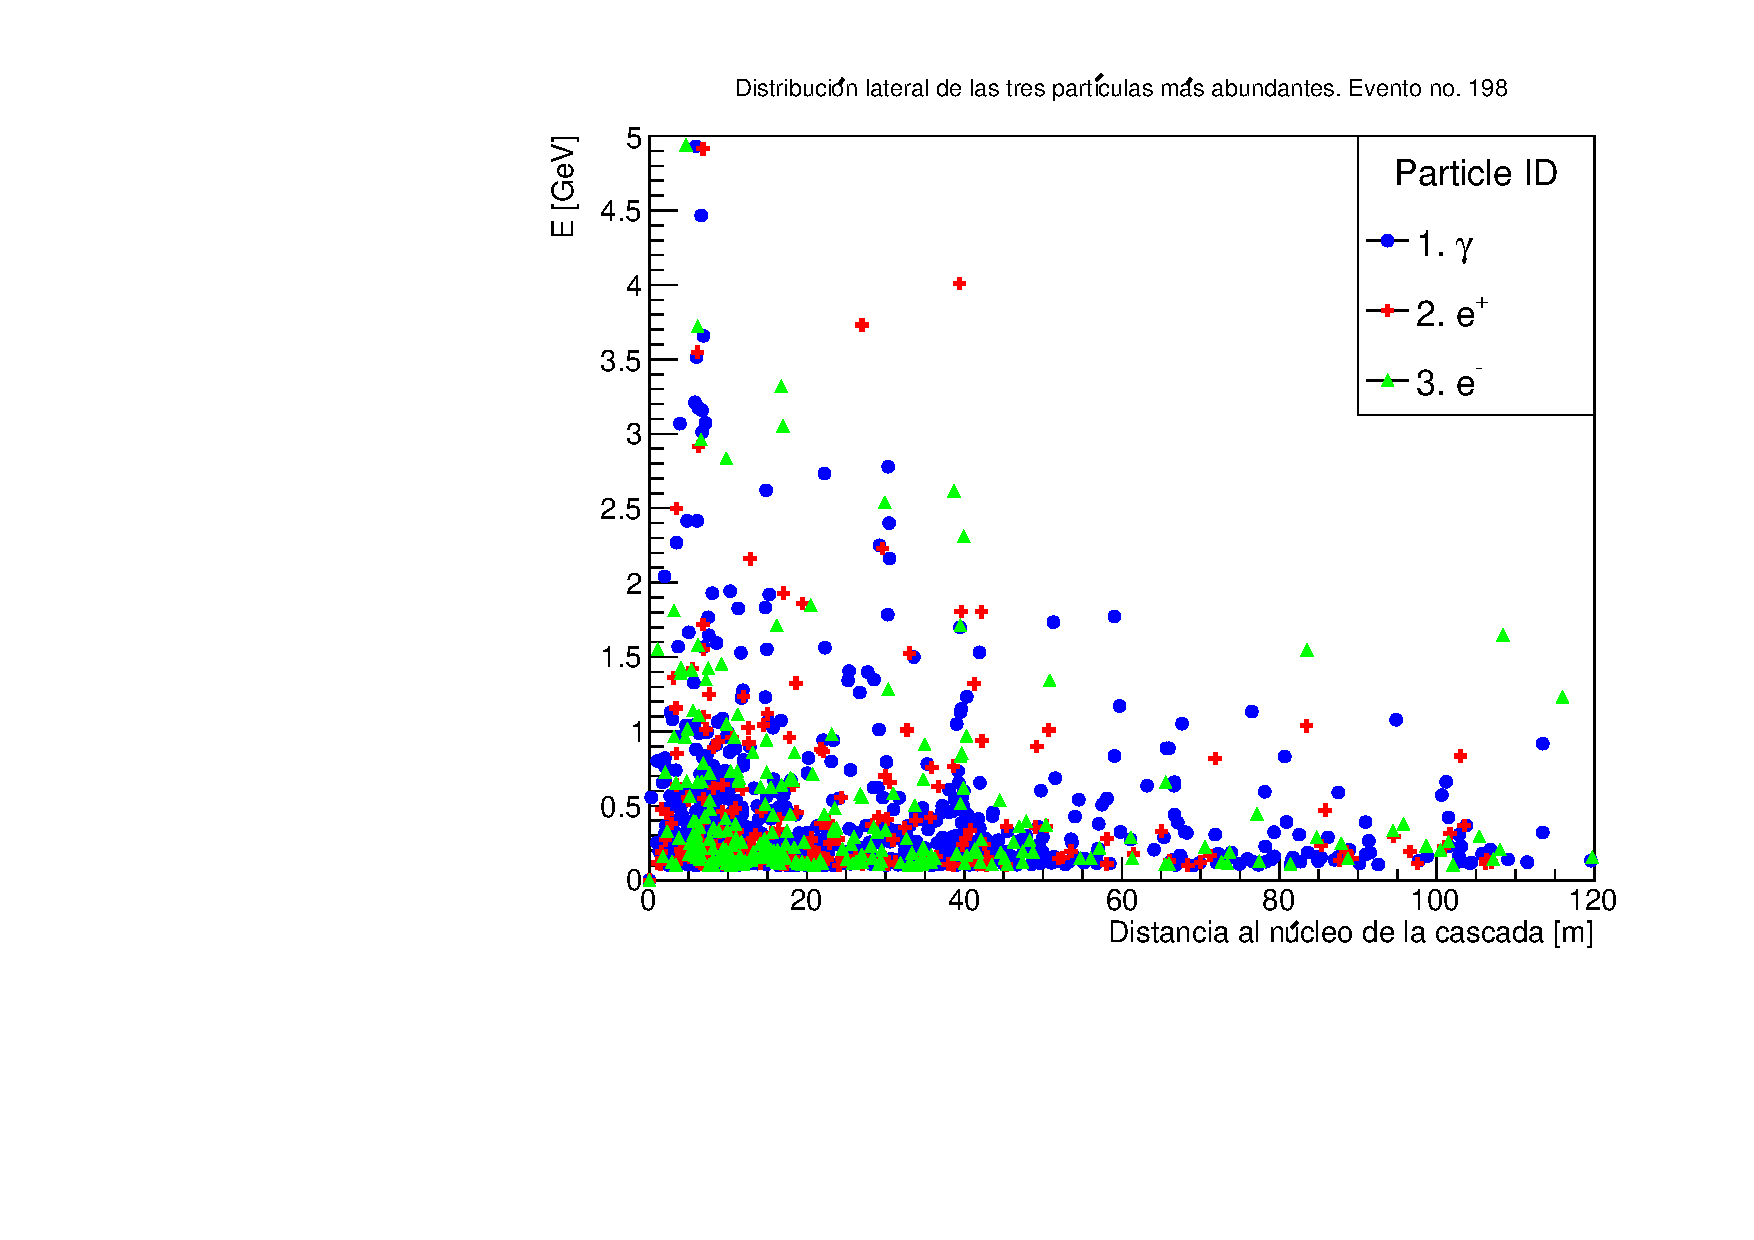
\includegraphics[width=0.9\textwidth]{../Figuras/Prob2D.pdf}
\caption{Distribución lateral para las tres partículas más abundantes, evento 198.}
\label{fig:Prob2B}
\end{figure}
\pagebreak
%%%%%%%%%%%%%%%%%%%%%%%%%%%%%%%%%%%%%%%%%%%%%%%%
\textbf{3)}
\begin{figure}[H]
\centering
\subfloat[\centering Distribución angular $\theta$]{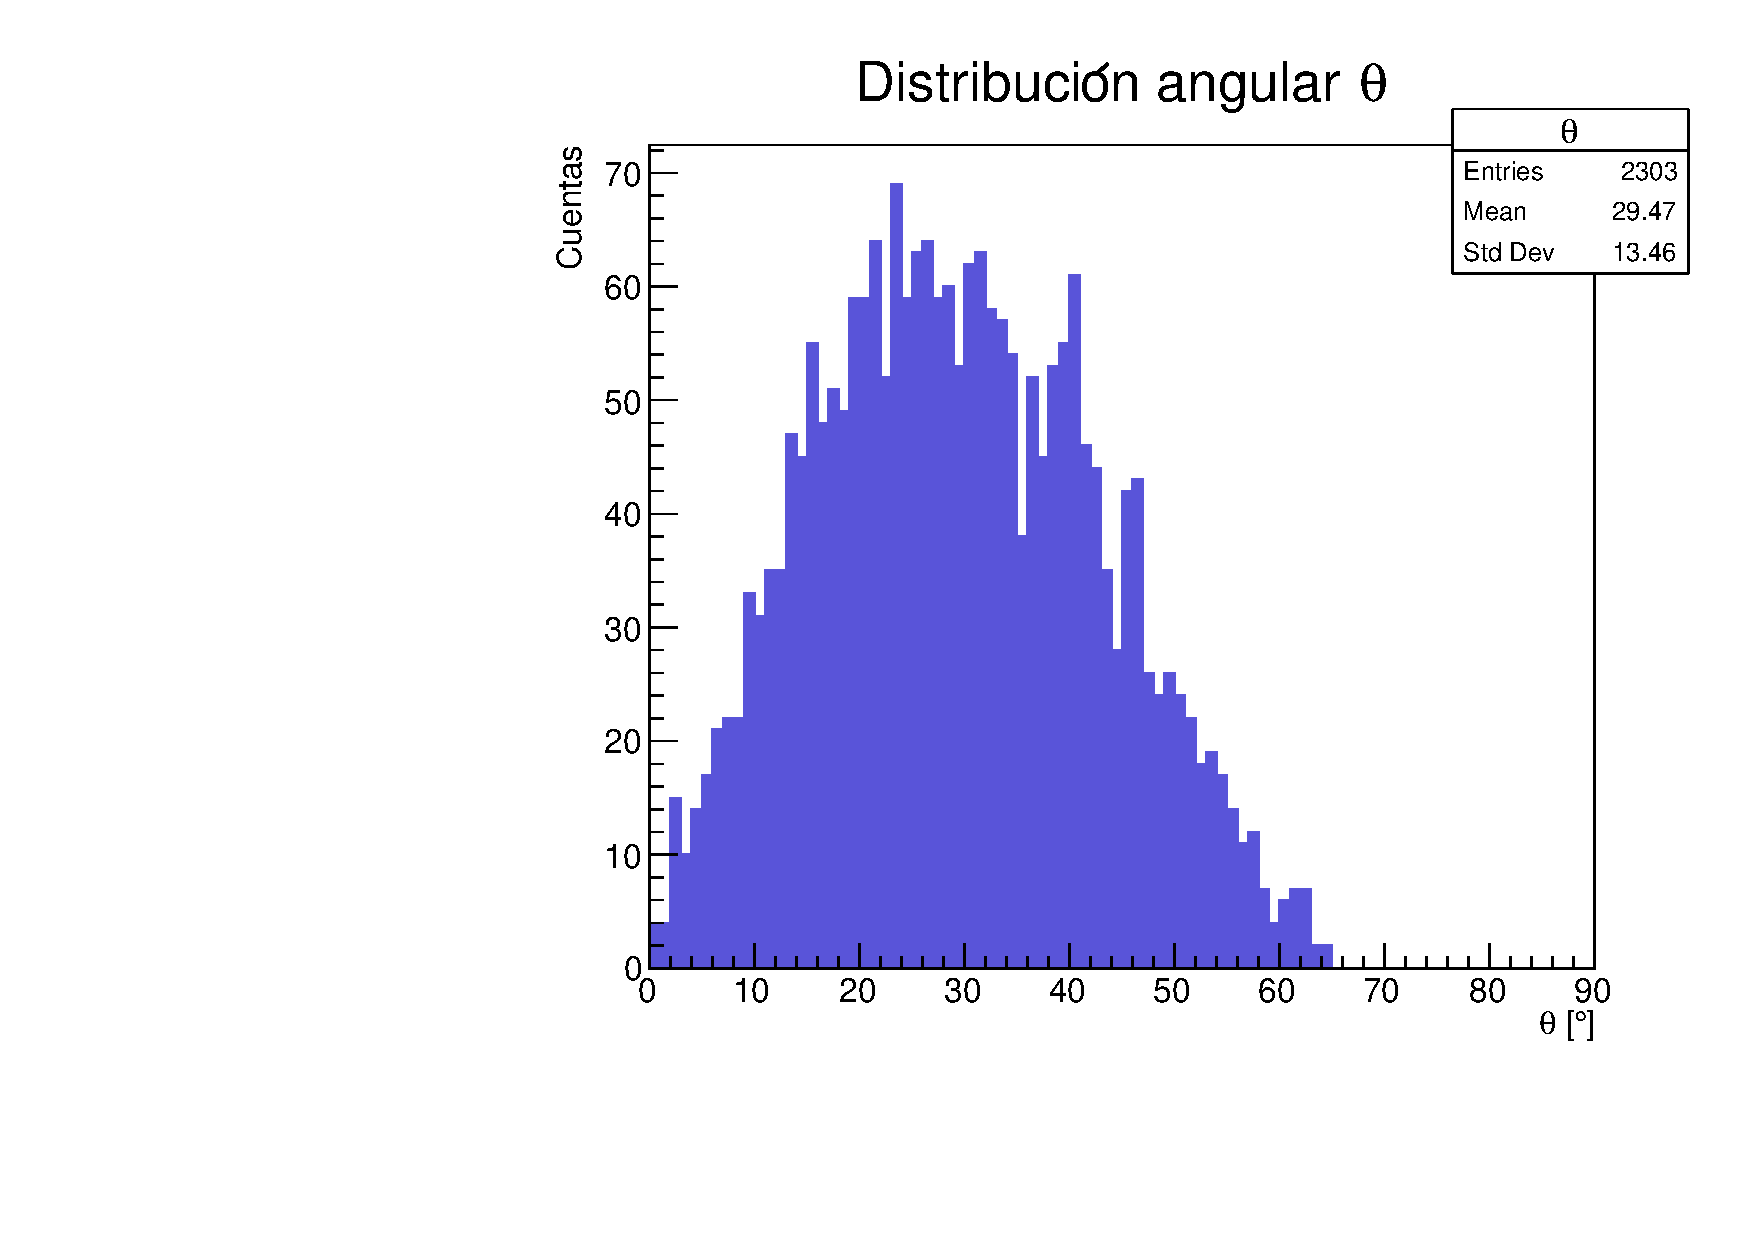
\includegraphics[width=0.68\textwidth]{../Figuras/Prob3A.pdf}}

\subfloat[\centering Distribución angular $\phi$]{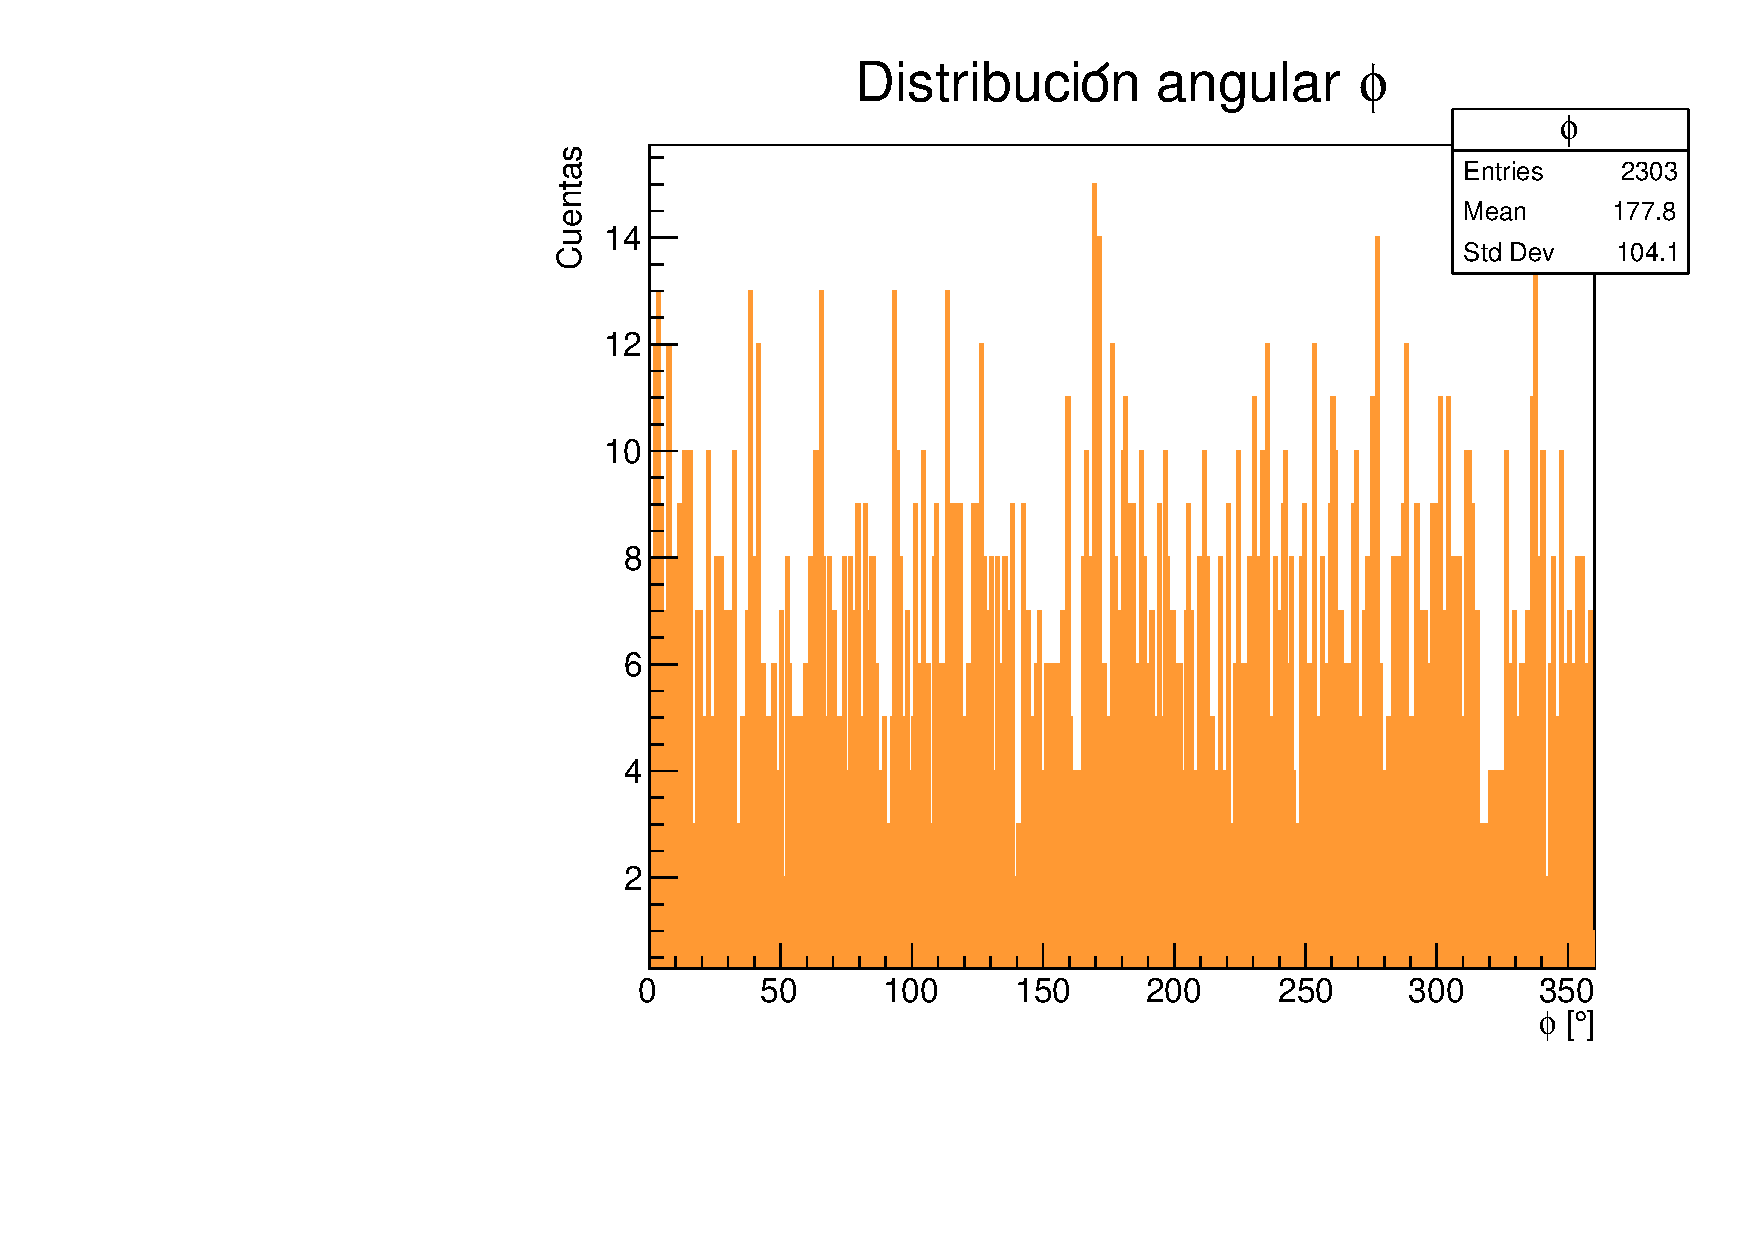
\includegraphics[width=0.68\textwidth]{../Figuras/Prob3B.pdf}}
\caption{Distribuciones angulares}
\label{fig:Prob3}
\end{figure}
Para saber si las distribuciones son o no razonables debemos comparar las gráficas con datos experimentales, al menos de manera cualitativa. En la tarea 6 se mostraron las distribuciones del ángulo cenital y el ángulo azimutal de las cascadas atmosféricas que se detectan en HAWC. Ahí, se apreciaba que para el ángulo cenital había un pico entre los 20° y 30° aproximadamente. En la figura \ref{fig:Prob3} (a) se alcanza a ver que en la distribución para $\theta$ obtenida con las simulaciones, se empieza a formar un pico en en la región antes mencionada; sin embargo, la curva no es tan suave como con los datos experimentales reales. Aún así, cualitativamente este resultado es razonable  considerando la baja estadística de las simulaciones. 

\hspace{5mm}Por otro lado, para $\phi$ observamos una distribución que si bien no es uniforme, no parece tener una región angular preferencial. Esto hecho sí contrasta con los datos experimentales, pues, nuevamente, en la tarea 6 se observó que el ángulo azimutal no tenía una distribución uniforme, sino que había dos regiones en las que había picos pronunciados debido a que el campo magnético de la Tierra desvía algunas partículas, dando lugar a zonas angulares $\phi$ en donde se detectan más partículas. En la figura \ref{fig:Prob3} (b) no se observa esto, por lo que el resultado en ese caso no es tan bueno y podría hacer falta más estadística.

\textbf{4)}
\begin{figure}[H]
\centering
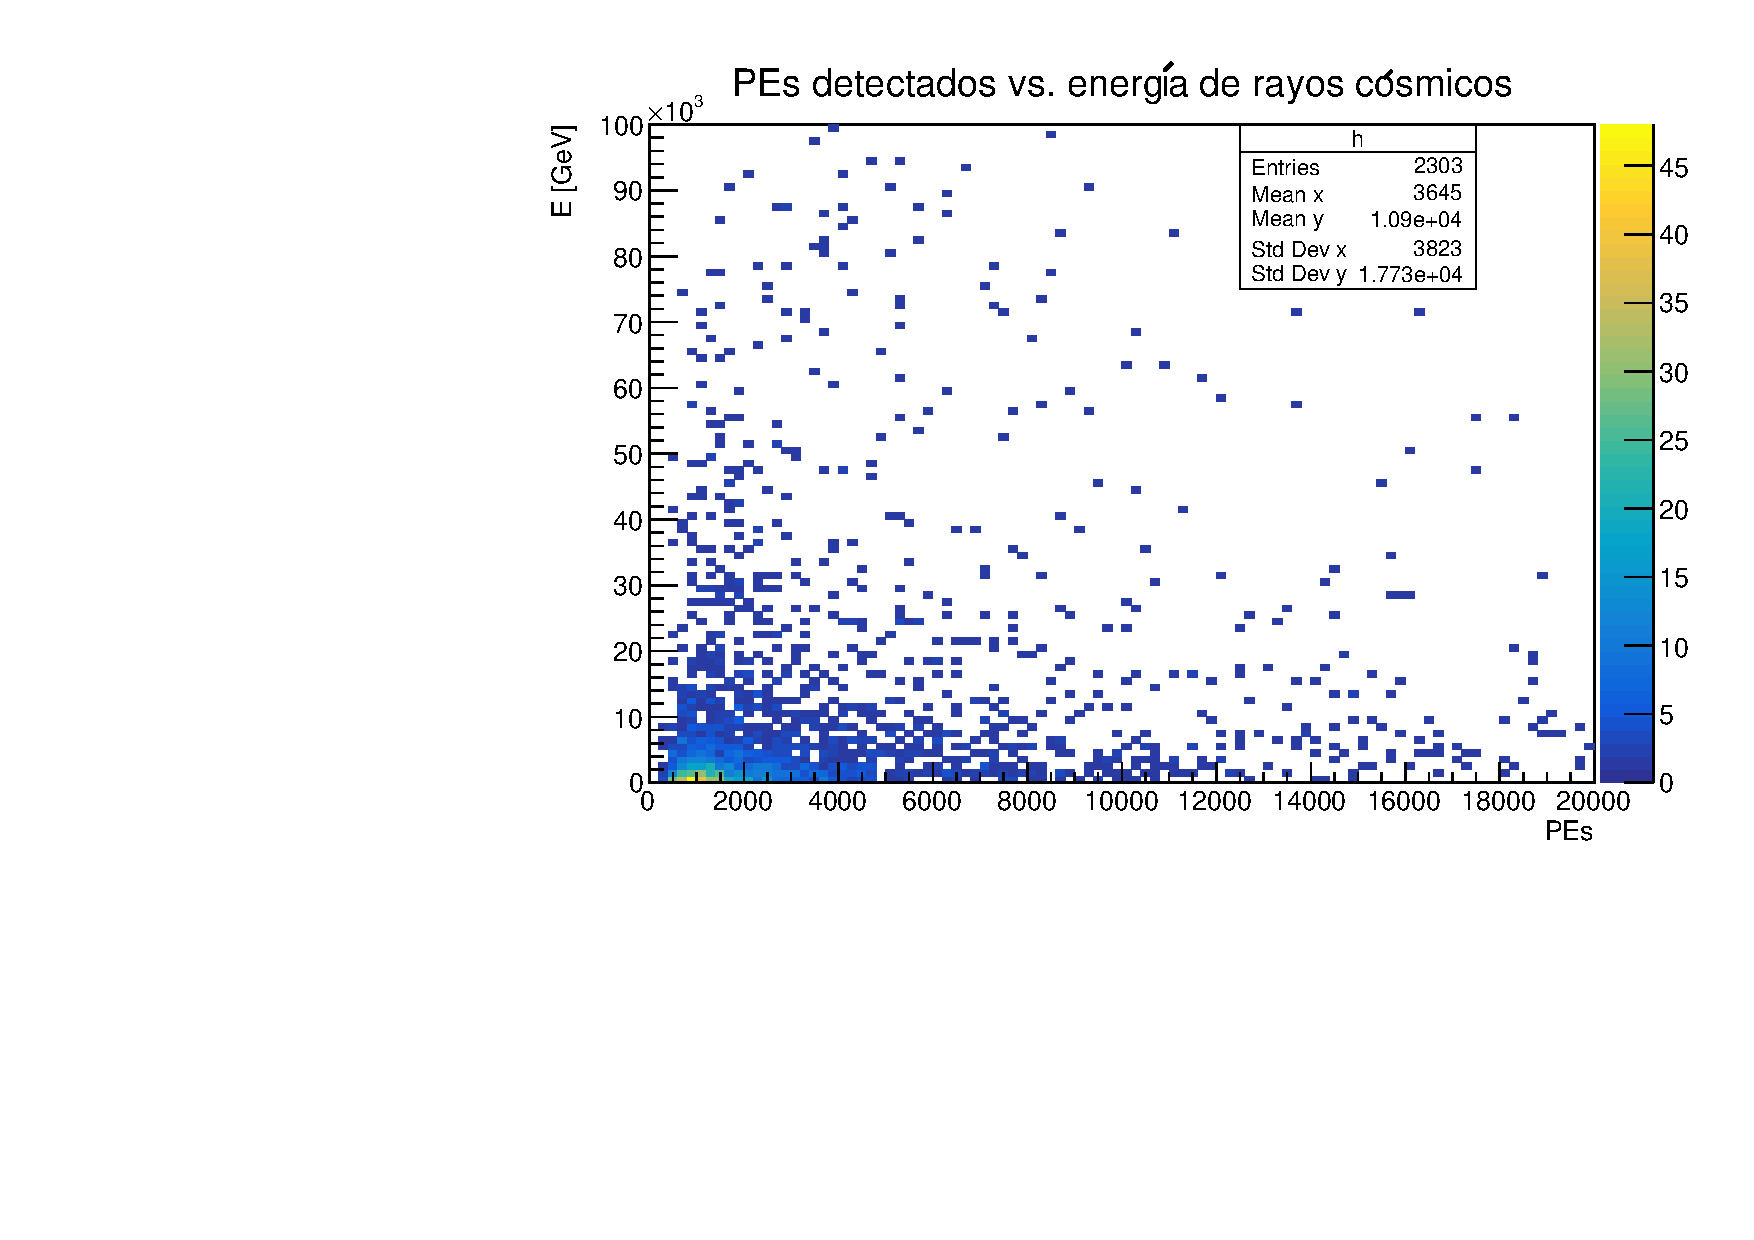
\includegraphics[width=1\textwidth]{../Figuras/Prob4A.pdf}
\caption{Número de PEs detectados vs. valor de la energía del rayo cósmico primario. La barra de colores nos indica el número de eventos detectados con las características correspondientes al eje $X$ y $Y$}
\label{fig:Prob4}
\end{figure}

En la figura \ref{fig:Prob4}, se observa que hay eventos en los cuales hay alta energía (mayor a $10^4$ GeV) con pocos PEs, pero también hay eventos en los que hay baja energía con pocos PEs, lo cual no da una relación bien determinada entre estos dos y nos llevaría a concluir que el número de PEs detectados no funciona como un estimador de energía. Sin embargo, la mayoría de los puntos que aparecen en la figura se encuentran con color azul marino, que indica pocas cuentas o pocos eventos con las características correspondientes a su posición en el histograma 2D. En la figura se aprecia que la mayoría de los eventos tienen pocos PEs (menos que 2,000) y bajas energías (menores a $10^4$ GeV), por lo que si despreciamos todos los demás eventos que no sean tan comunes (los que son de azul marino), pudiese ser que la gráfica anterior funcionase como un estimador de la energía.





\end{document}